\documentclass{beamer}

% Tema de beamer
\usetheme{AnnArbor}

% Paquetes
\usepackage[utf8]{inputenc}
\usepackage[spanish]{babel}
\usepackage{pifont}

% Datos de la presentación
\title{Exposición del CV, proyecto y programa}
\subtitle{Concurso plaza PPL–003–25}
\author{Mario Gómez Ramos}
\institute[]{Universidad de Sevilla \\ Departamento de Física Atómica Molecular y Nuclear \\ Grupo de Física Nuclear Básica}
\date{\today}

\AtBeginSection[]{
  \begin{frame}{Contenido}
    \tableofcontents[currentsection]
  \end{frame}
}

\begin{document}

% Portada
\begin{frame}
    \titlepage
\end{frame}

% Tabla de contenidos
\begin{frame}{Contenido}
    \tableofcontents
\end{frame}

% Sección 1: Curriculum Vitae
\section{Curriculum Vitae}
\subsection{Formación}
\begin{frame}{Formación}
    \begin{itemize}
        \item Licenciado en Física \hfill 2008-2013 \\ Universidad de Sevilla \\ Nota media: 9.68/10 (Premio Nacional en Física)\\
        
        \item Máster Interuniversitario en Física Nuclear \hfill 2013-2014 \\ US, UAM, UB, UCM, UGR, USAL \\ Nota media: 9.6/10 (Premio extraordinario)\\
        \item Doctor en Ciencias y Tecnologías Físicas \hfill 2014-2018 \\Universidad de Sevilla \\ Nota: Sobresaliente cum laude\\
    \end{itemize}
\end{frame}

\subsection{Docencia}
\begin{frame}{Docencia}
    \begin{itemize}
        \item Horas impartidas (508.1 horas)
        \begin{itemize}
        \item Predoctorales (Universidad de Sevilla): 120 horas
        \item Postdoctorales (Universidad de Sevilla): 388.1 horas (40.6 TFG y TFM)
        \end{itemize}
    \item Experiencia en Física Nuclear y de Partículas (161.5 horas) e Introducción a las reacciones nucleares (56 horas)
    \item Dirección de TFGs (6) y TFMs (1)
    \item Informes favorables de la labor docente
    \end{itemize}
\end{frame}

\subsection{Investigación}
\begin{frame}{Investigación}
    \begin{itemize}
        \item Resumen Scopus:
        \begin{center}
        \begin{tabular}{cccc}
        Nº pub.: 37 & Nº citas: 419 & Media citas: 11,32 & Índice h: 12\\
        \tiny Q1:26 (81\%) SCIJR &&&
        \end{tabular}
        \end{center}
        \item Beca Humboldt para Investigadores Jóvenes ($\sim$2 años TU Darmstadt) y contrato JdC Incorporación
    \item Participación en 9 proyectos de investigación
        \item Estancias en RCNP y U. Surrey  

    \item Intensa actividad como referee    
    \item Participación en reuniones científicas:  
    \begin{itemize}
    \item 1 charla invitada
    \item 12 ponencias orales
    \item 3 pósters
    \end{itemize}
    \item Co-organizador de Nuclear Reaction Seminars: \url{https://reactionseminar.github.io/}
    \item Actividades de divulgación y transferencia (EUROLABS)
    \end{itemize}
\end{frame}

% Sección 2: Proyecto
\section{Proyecto}
\subsection{Planteamientos investigadores}
\begin{frame}{Planteamientos investigadores}
    \begin{block}{Perfil investigador}
       Estudio teórico de reacciones nucleares directas a energías bajas e intermedias.
    \end{block}
    \begin{center}
    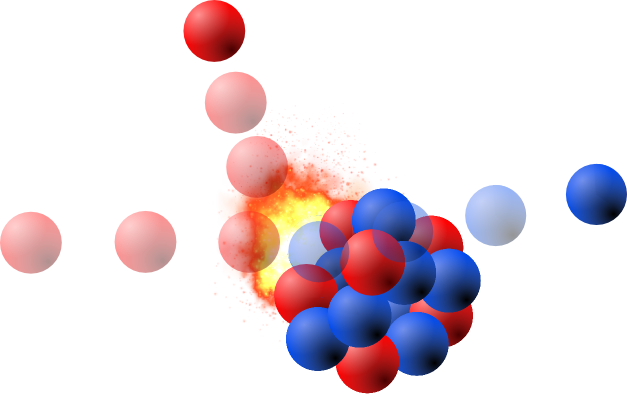
\includegraphics[width=0.6\textwidth]{portada.png}
    \end{center}
\end{frame}

%\begin{frame}{Planteamientos investigadores}

%    \textbf{Reacciones nucleares}    
    
%    \begin{itemize}
%    \item Astrofísica (nucleosíntesis) \hfill 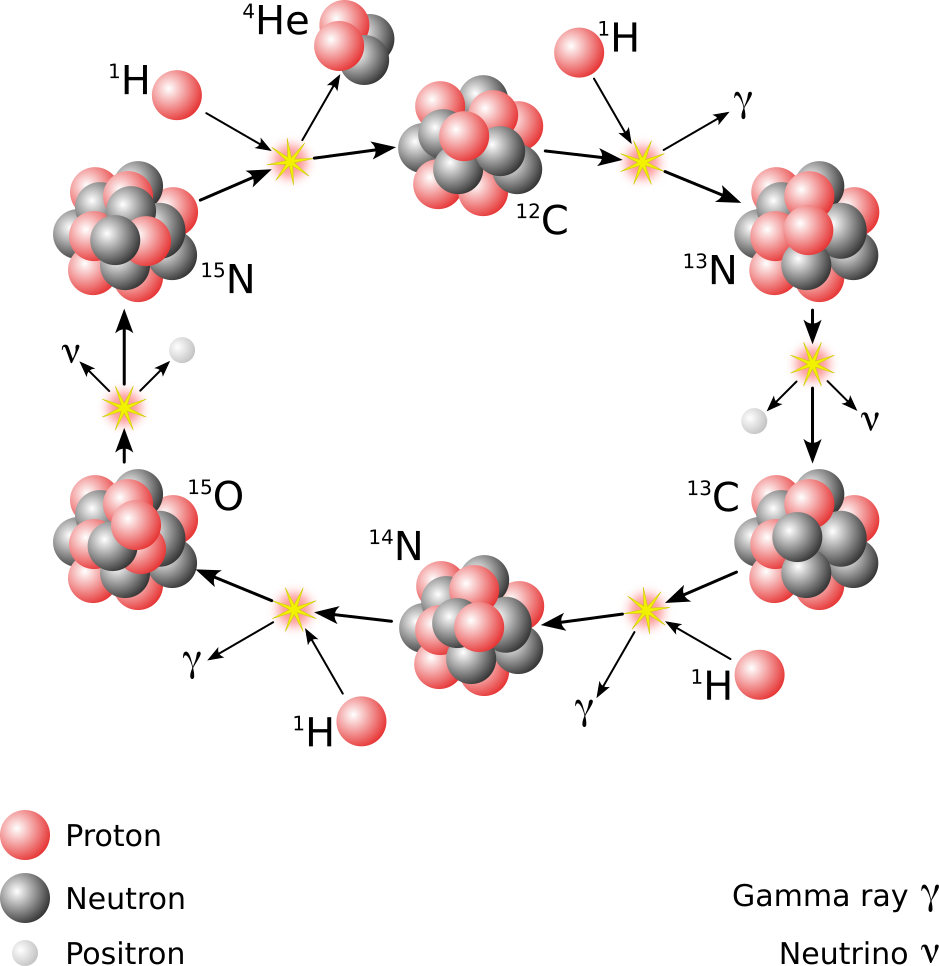
\includegraphics[width=0.15\textwidth]{CNO_cycle.png}
    
%    \item Radiomedicina \hfill  \includegraphics[width=0.15\textwidth]{protontherapy.png}
    
%    \item Producción de energía \hfill  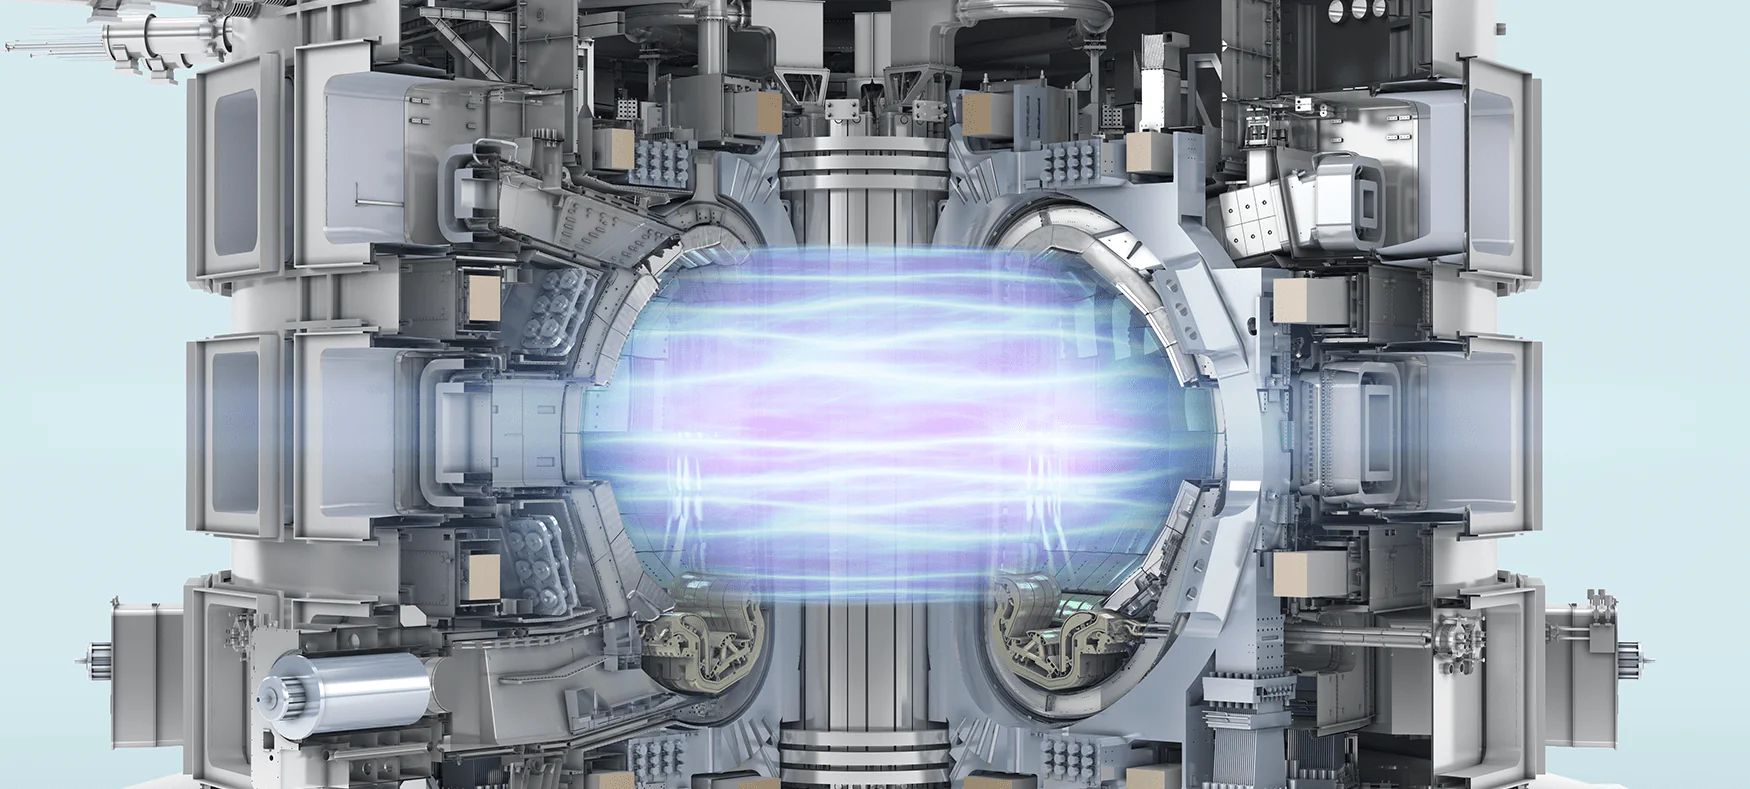
\includegraphics[width=0.15\textwidth]{fusion.png}
    
%    \item Investigación básica (núcleos exóticos)\hfill  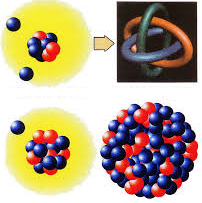
\includegraphics[width=0.15\textwidth]{exotic.png}
%    \end{itemize}
%\end{frame}

\begin{frame}{Reacciones nucleares y estructura nuclear} 
    \begin{center}
    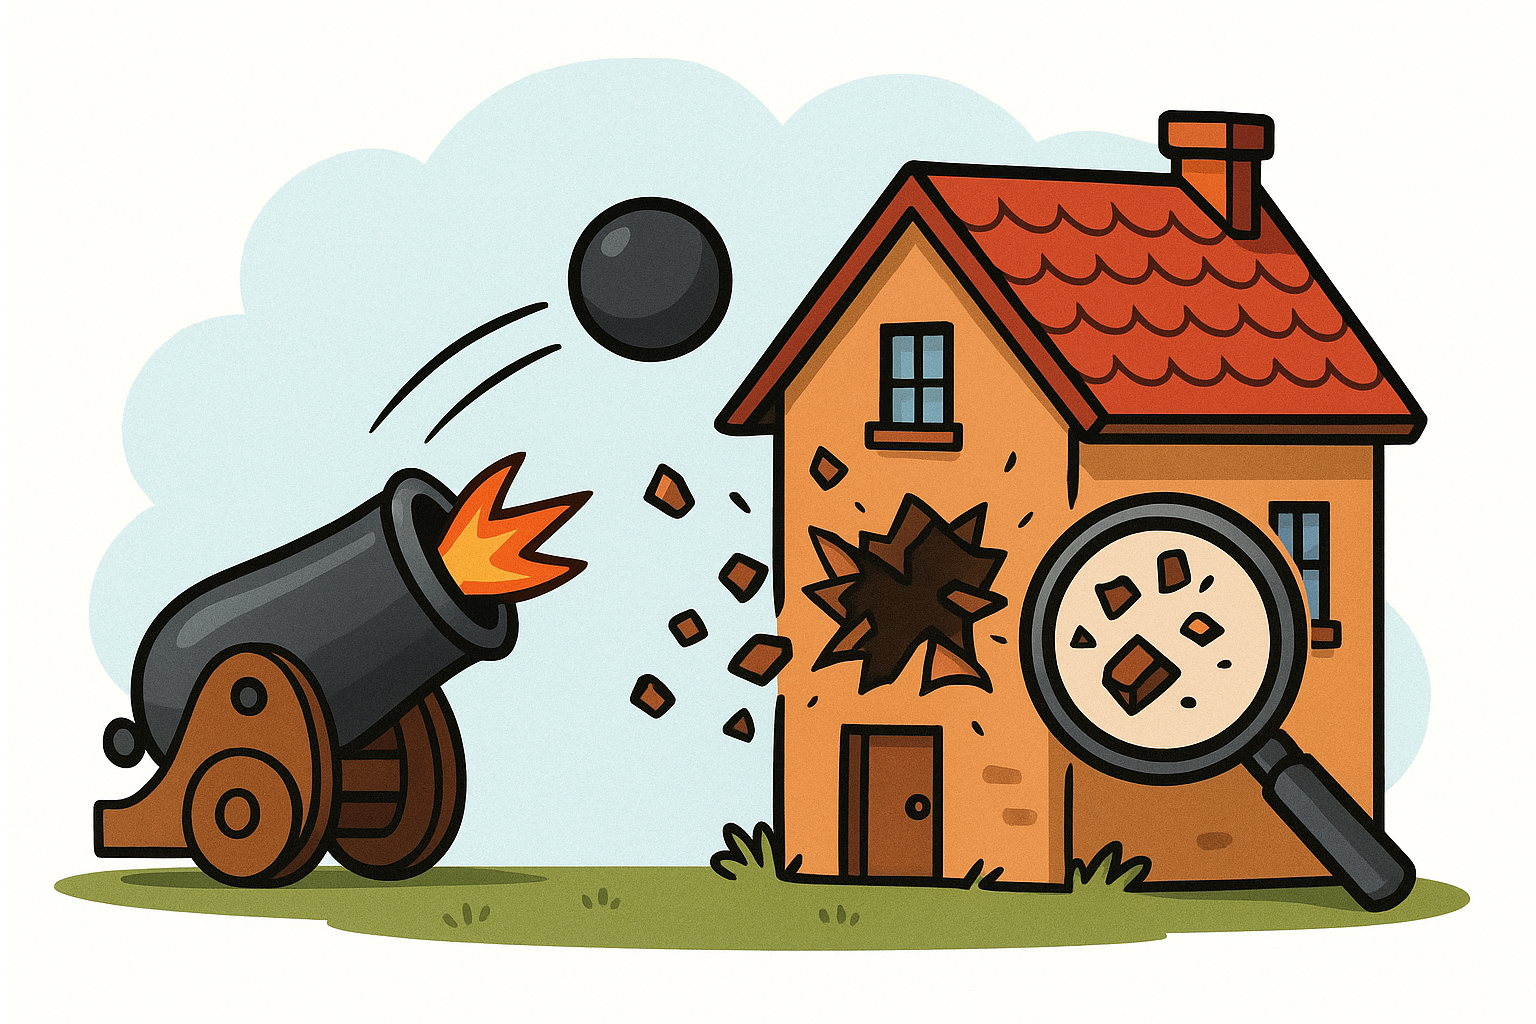
\includegraphics[width=0.4\textwidth]{cannon.png}
    \end{center}
    \begin{itemize}
    \item Reacciones directas: involucran menos grados de libertad (¿¿más sencillas??)
    \item Formalismo de reacción esencial para conseguir información fiable de los experimentos
    \end{itemize}
\end{frame}

\begin{frame}{Antecedentes: Quenching factors} 
    \begin{minipage}{0.45\textwidth}
    \begin{center}
    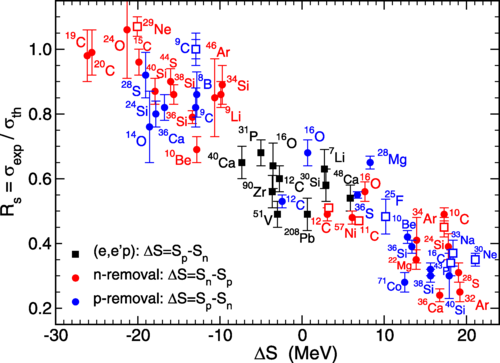
\includegraphics[height=0.4\textheight]{Tostevin.png}
    
    \tiny J.A.~Tostevin \& A.~Gade, PRC \textbf{103}, 054610 (2021)
   
  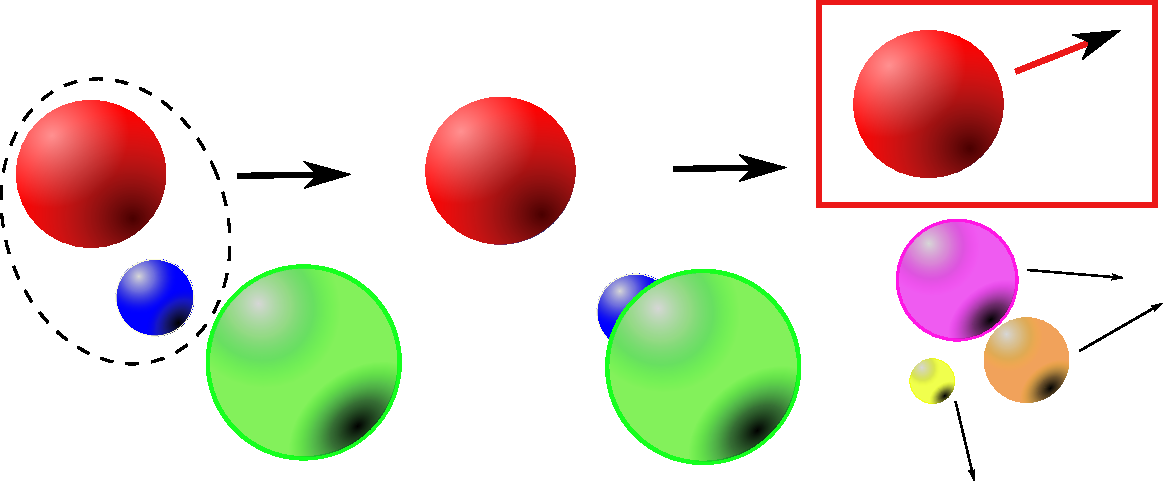
\includegraphics[height=0.3\textheight,width=\textwidth, keepaspectratio]{stripping.pdf}   
    \end{center}
    \end{minipage}
    \begin{minipage}{0.45\textwidth}
    \begin{center}
    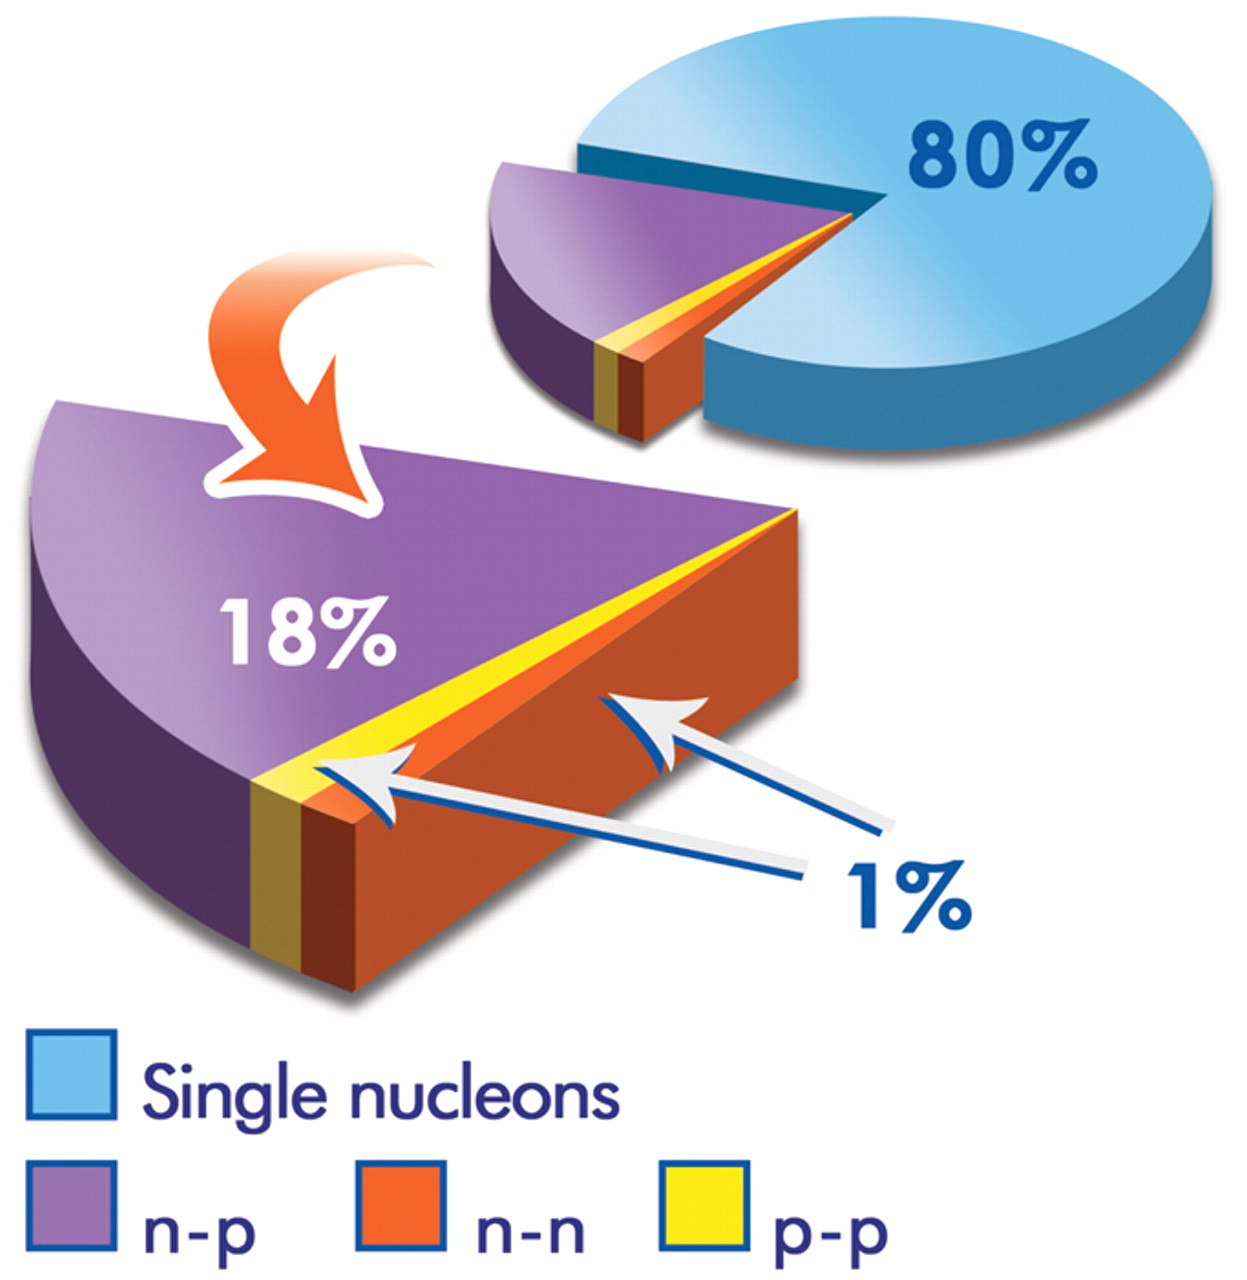
\includegraphics[height=0.4\textheight]{subedi.jpeg}
    
    \tiny R.~Subedi \textit{et al}, Science \textbf{320}, 1476 (2008)
    \end{center}
    \end{minipage}
    \begin{itemize}
    \item Más correlaciones de la especie escasa?
    \end{itemize}
    
\end{frame}

\begin{frame}{Antecedentes: Quenching factors} 
    \begin{minipage}{0.45\textwidth}
    \begin{center}
    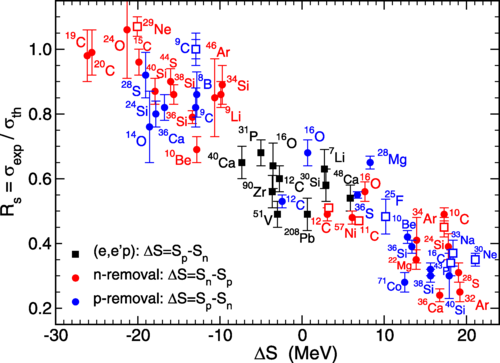
\includegraphics[height=0.4\textheight]{Tostevin.png}
    
    \tiny J.A.~Tostevin \& A.~Gade, PRC \textbf{103}, 054610 (2021)

  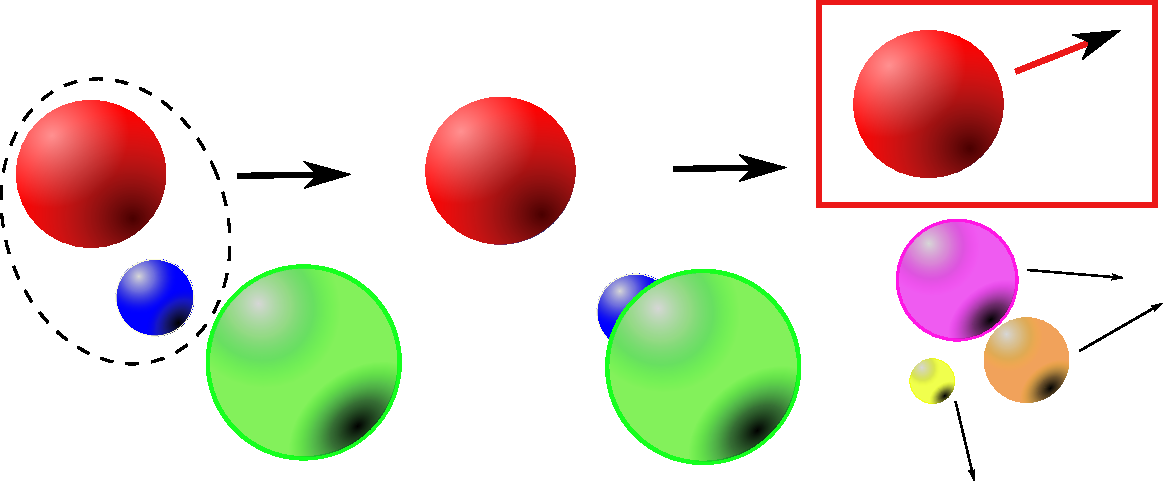
\includegraphics[height=0.3\textheight,width=\textwidth, keepaspectratio]{stripping.pdf}   
    \end{center}
    \end{minipage}
    \begin{minipage}{0.45\textwidth}
    \begin{center}
    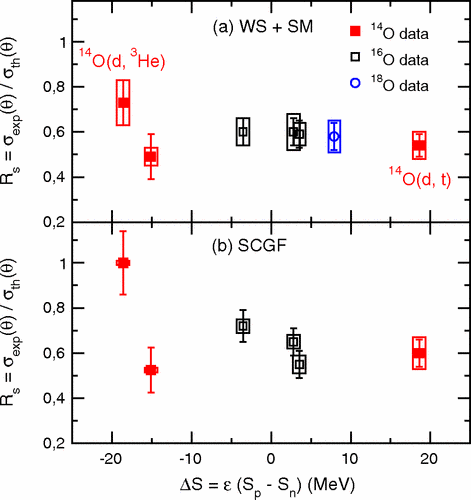
\includegraphics[height=0.4\textheight]{flavigny.png}
    
    \tiny F.~Flavigny \textit{et al}, PRL \textbf{110}, 122503 (2013)

    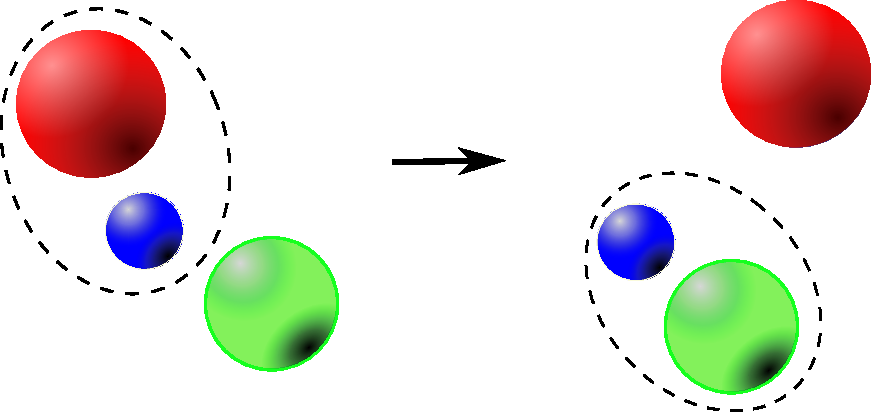
\includegraphics[height=0.3\textheight,width=\textwidth, keepaspectratio]{transfer.pdf}
    \end{center}
    \end{minipage}
    \begin{itemize}
    \item Resultados inconsistentes entre dos tipos de reacciones
    \end{itemize}
    
\end{frame}

\begin{frame}{Antecedentes: Quenching factors} 
    \begin{minipage}{0.45\textwidth}
    \begin{center}
    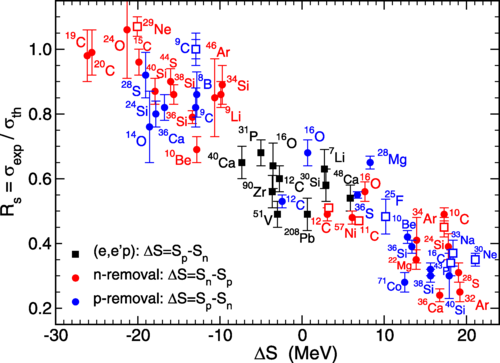
\includegraphics[height=0.3\textheight]{Tostevin.png}
    
    \tiny J.A.~Tostevin \& A.~Gade, PRC \textbf{103}, 054610 (2021)
    \end{center}
    \end{minipage}
    \begin{minipage}{0.45\textwidth}
    \begin{center}
    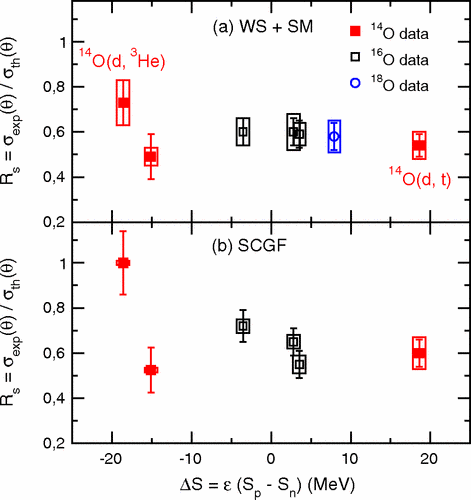
\includegraphics[height=0.3\textheight]{flavigny.png}
   
        \tiny F.~Flavigny \textit{et al}, PRL \textbf{110}, 122503 (2013)
    \end{center}
    \end{minipage}

    \begin{minipage}{0.45\textwidth}
    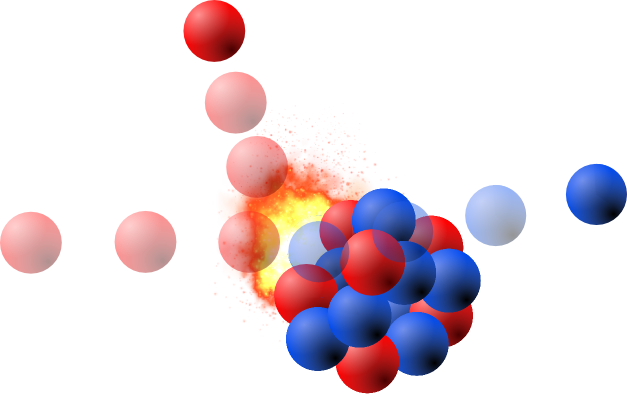
\includegraphics[height=0.3\textheight]{portada.png}
    \end{minipage}
    \begin{minipage}{0.45\textwidth}
    \begin{center}
    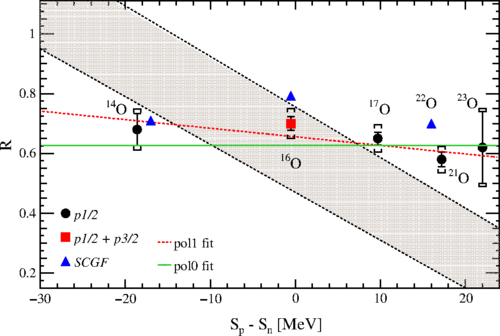
\includegraphics[height=0.3\textheight]{atar.png}
   
        \tiny L.~Atar \textit{et al}, PRL \textbf{120}, 052501 (2018)
    \end{center}
    \end{minipage}


\begin{itemize}
\item $(p,2p)$ concuerda con transferencia
\end{itemize}
    
\end{frame}

\begin{frame}{Antecedentes: Instalaciones de haces de núcleos exóticos} 
    \begin{minipage}{0.45\textwidth}
    \begin{center}
    
\includegraphics[height=0.3\textheight]{fair.jpg}
    \end{center}
    \end{minipage}
    \begin{minipage}{0.45\textwidth}
    \begin{center}
    
\includegraphics[height=0.3\textheight]{frib.jpg}
    \end{center}
    \end{minipage}

    \begin{minipage}{0.45\textwidth}
    \begin{center}
    
\includegraphics[height=0.15\textheight, width=\textwidth, keepaspectratio]{riken.png}
    \vspace{0.3cm}
    
\includegraphics[height=0.15\textheight, width=\textwidth, keepaspectratio]{onokoro.png}
    \end{center}
    \end{minipage}
    \begin{minipage}{0.45\textwidth}
    \begin{center}
    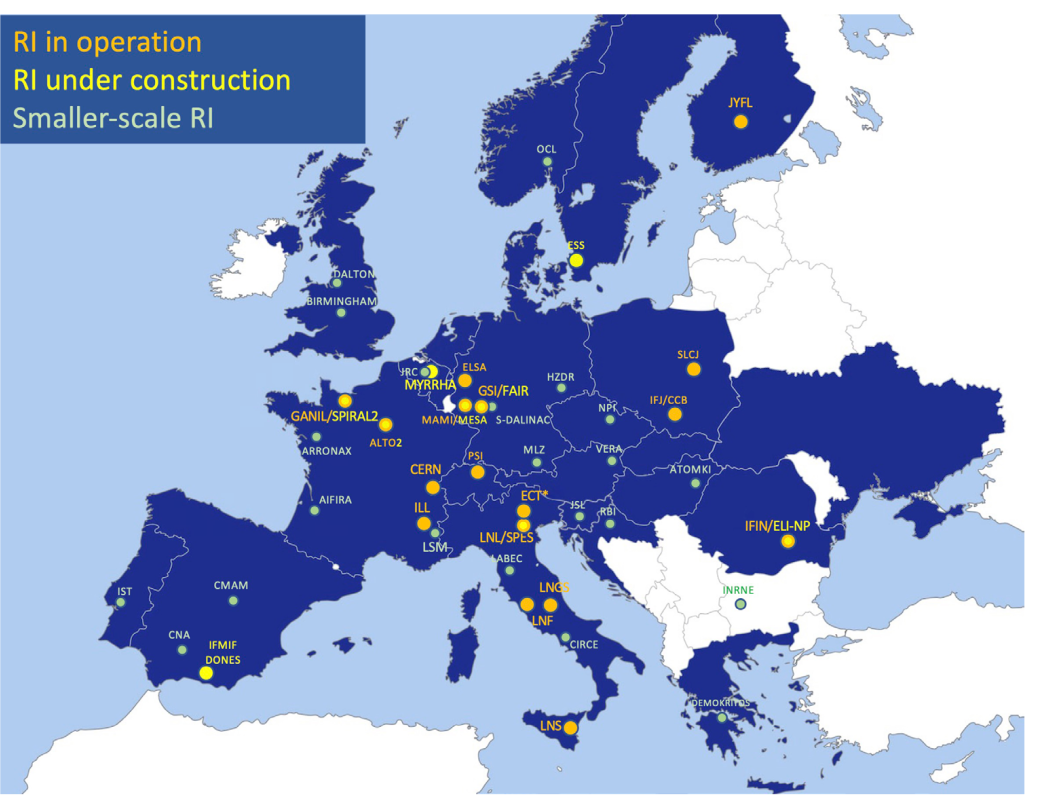
\includegraphics[height=0.3\textheight]{EuRI.png}
    \end{center}
    \end{minipage}
    
    \begin{itemize}
    \item Interés en correlaciones nucleón-nucleón
    \item Blancos de hidrógeno activos y líquidos serán usados extensivamente
    \item Interés en consistencia entre reacciones y estructura nuclear
    \end{itemize}
\end{frame}

%\begin{frame}{Experiencia previa} 

%   \begin{minipage}{0.45\textwidth}
%   \ding{212} \tiny Reacciones de arranque de un nucleón (problema de los “quenching
%   factors”)
   
%    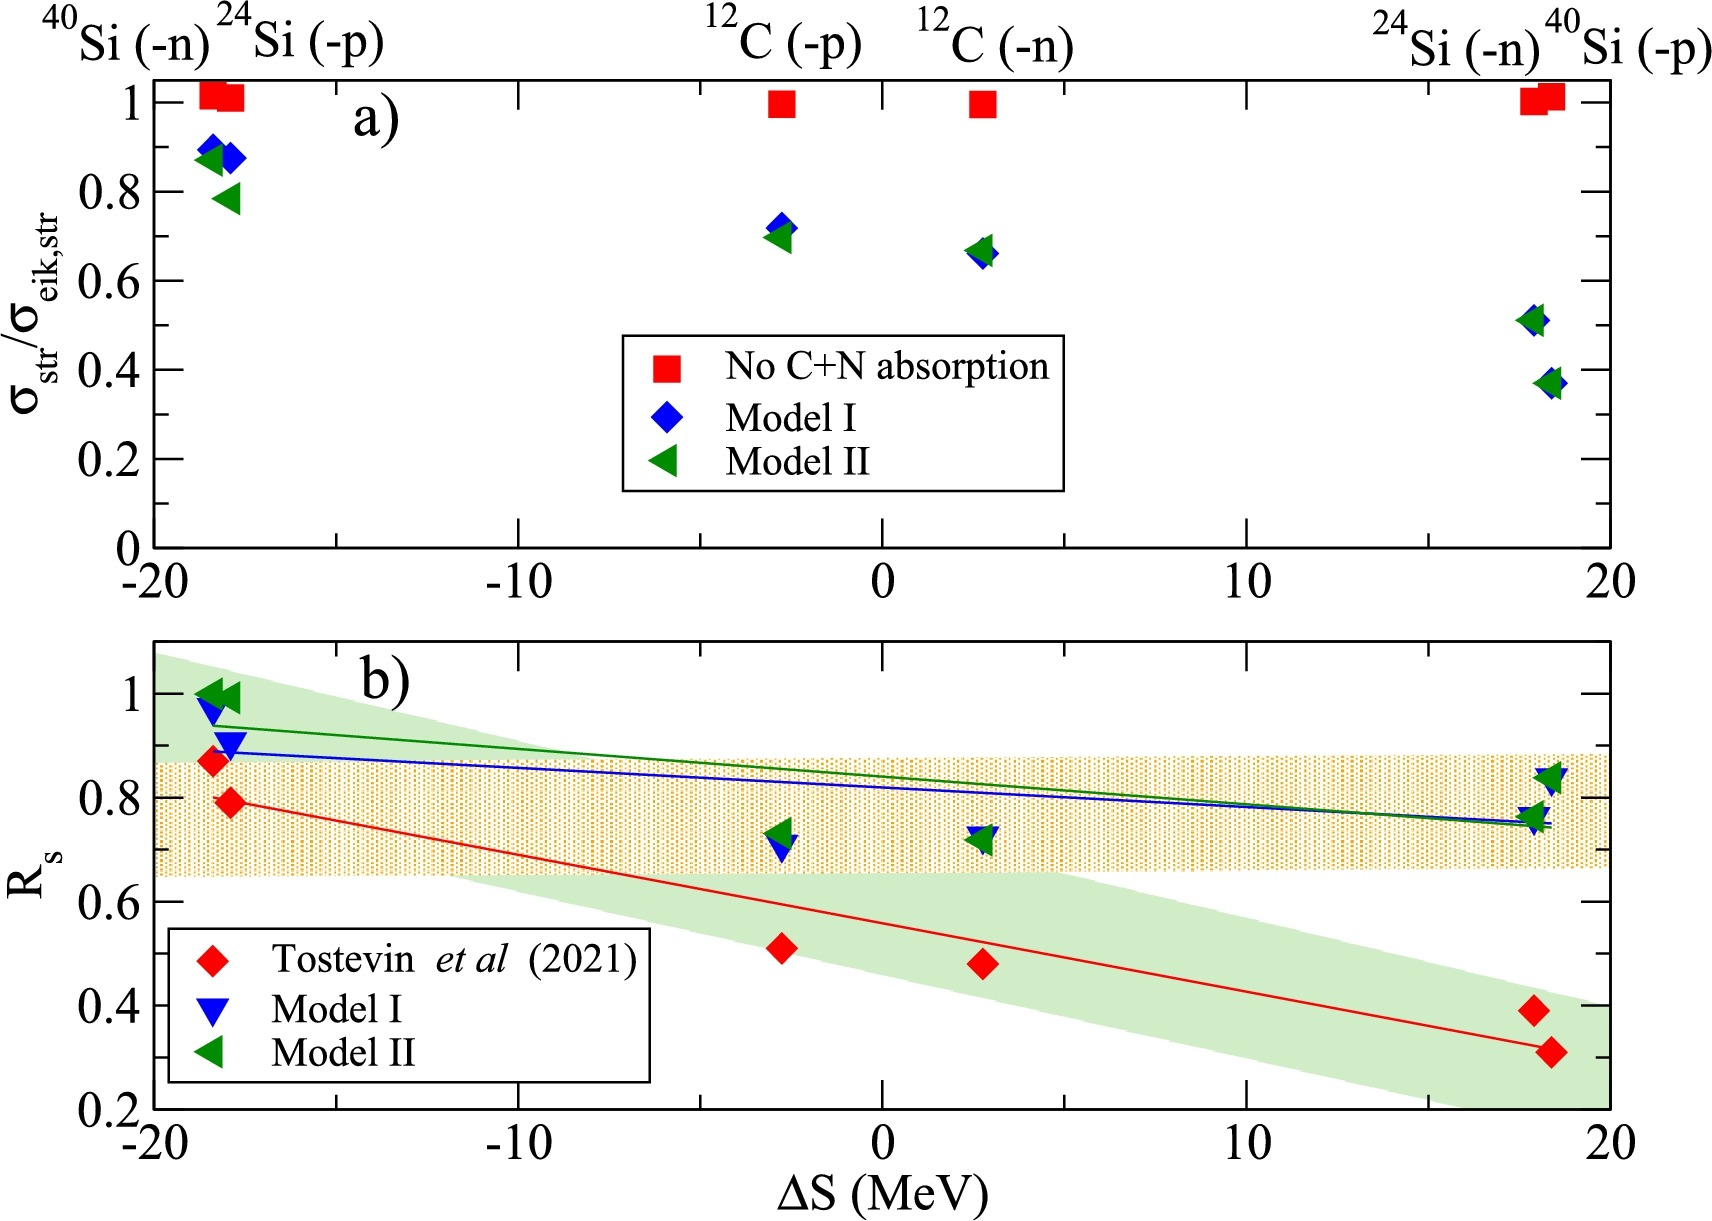
\includegraphics[height=0.3\textheight]{quenching.jpg}
%    \end{minipage}
%    \begin{minipage}{0.45\textwidth}
%    \ding{212} \tiny Correlaciones y reacciones de arranque de dos nucleones: reacciones $(p,3p)$
    
%    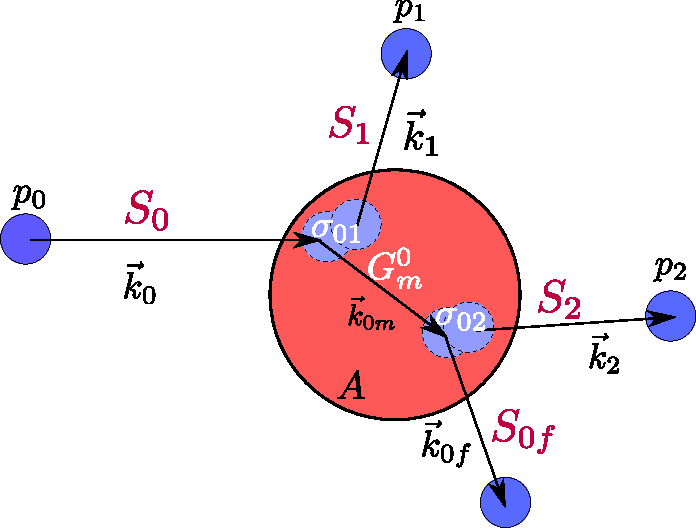
\includegraphics[height=0.3\textheight]{model.pdf}
    
%    \end{minipage}

%    \begin{center}
%    \begin{minipage}{0.45\textwidth}
%    \ding{212} \tiny Teorías a energías bajas (no-localidad, excitaciones colectivas)    
    
%    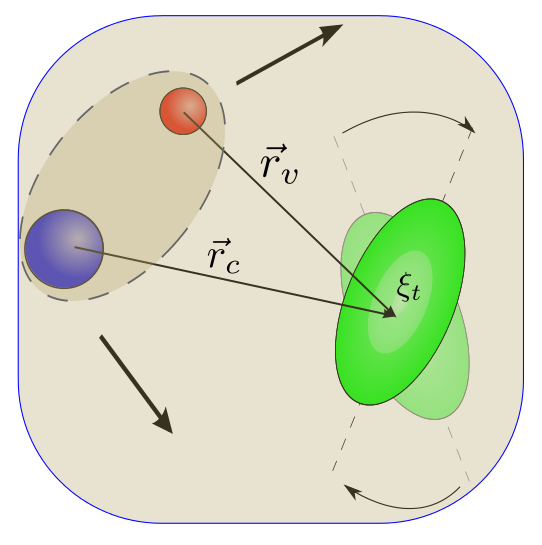
\includegraphics[height=0.3\textheight, width=\textwidth, keepaspectratio]{TExc.png}
%    \end{minipage}
%    \end{center}

    
%\end{frame}






\begin{frame}{Líneas de investigación} 

\large \ding{90}  L1: \underline{Reacciones de arranque de una partícula:} \underline{reacciones $(p, pN )$, knockout y transferencia}

\normalsize
    
   \fbox{ \begin{minipage}{0.45\textwidth}
    \begin{center}
    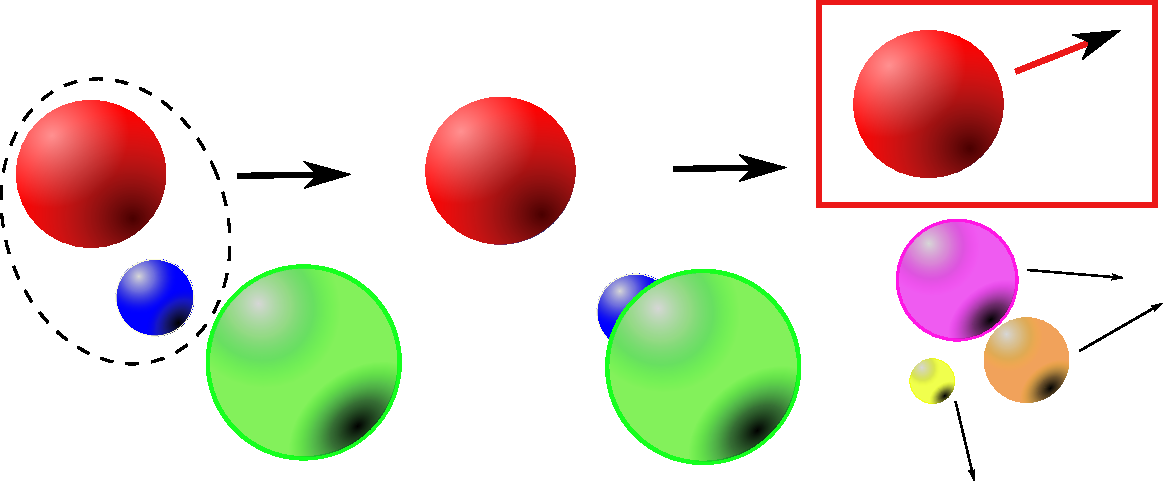
\includegraphics[height=0.3\textheight,width=\textwidth, keepaspectratio]{stripping.pdf}
\end{center}    
    \end{minipage}}
 \fbox{   \begin{minipage}{0.45\textwidth}
    \begin{center}
    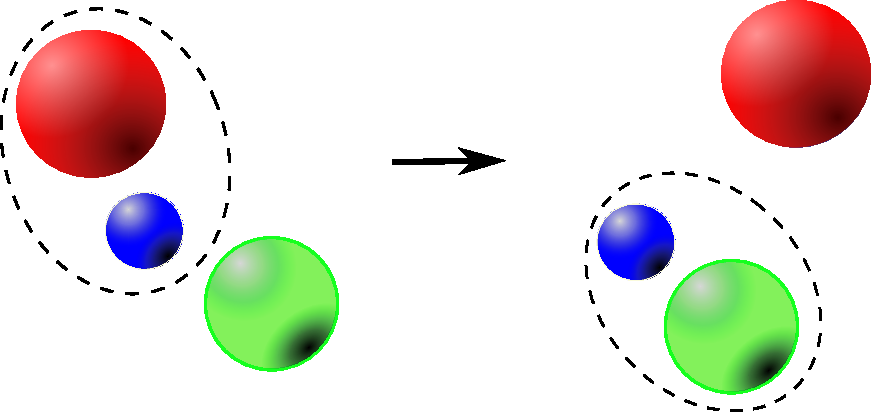
\includegraphics[height=0.3\textheight,width=\textwidth, keepaspectratio]{transfer.pdf}
    \end{center}
    \end{minipage}}

\begin{center}
   \fbox{ \begin{minipage}{0.45\textwidth}
    \begin{center}
    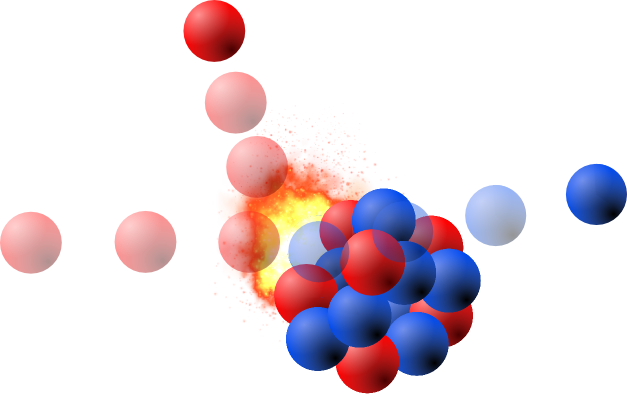
\includegraphics[height=0.3\textheight]{portada.png}
    \end{center}
    \end{minipage}}
\end{center}
    
\end{frame}

\begin{frame}{Experiencia previa} 

   \begin{minipage}{0.45\textwidth}
   \ding{212} \tiny L1: \underline{Reacciones de arranque de una partícula:} \underline{reacciones $(p, pN )$, knockout y transferencia}
   
    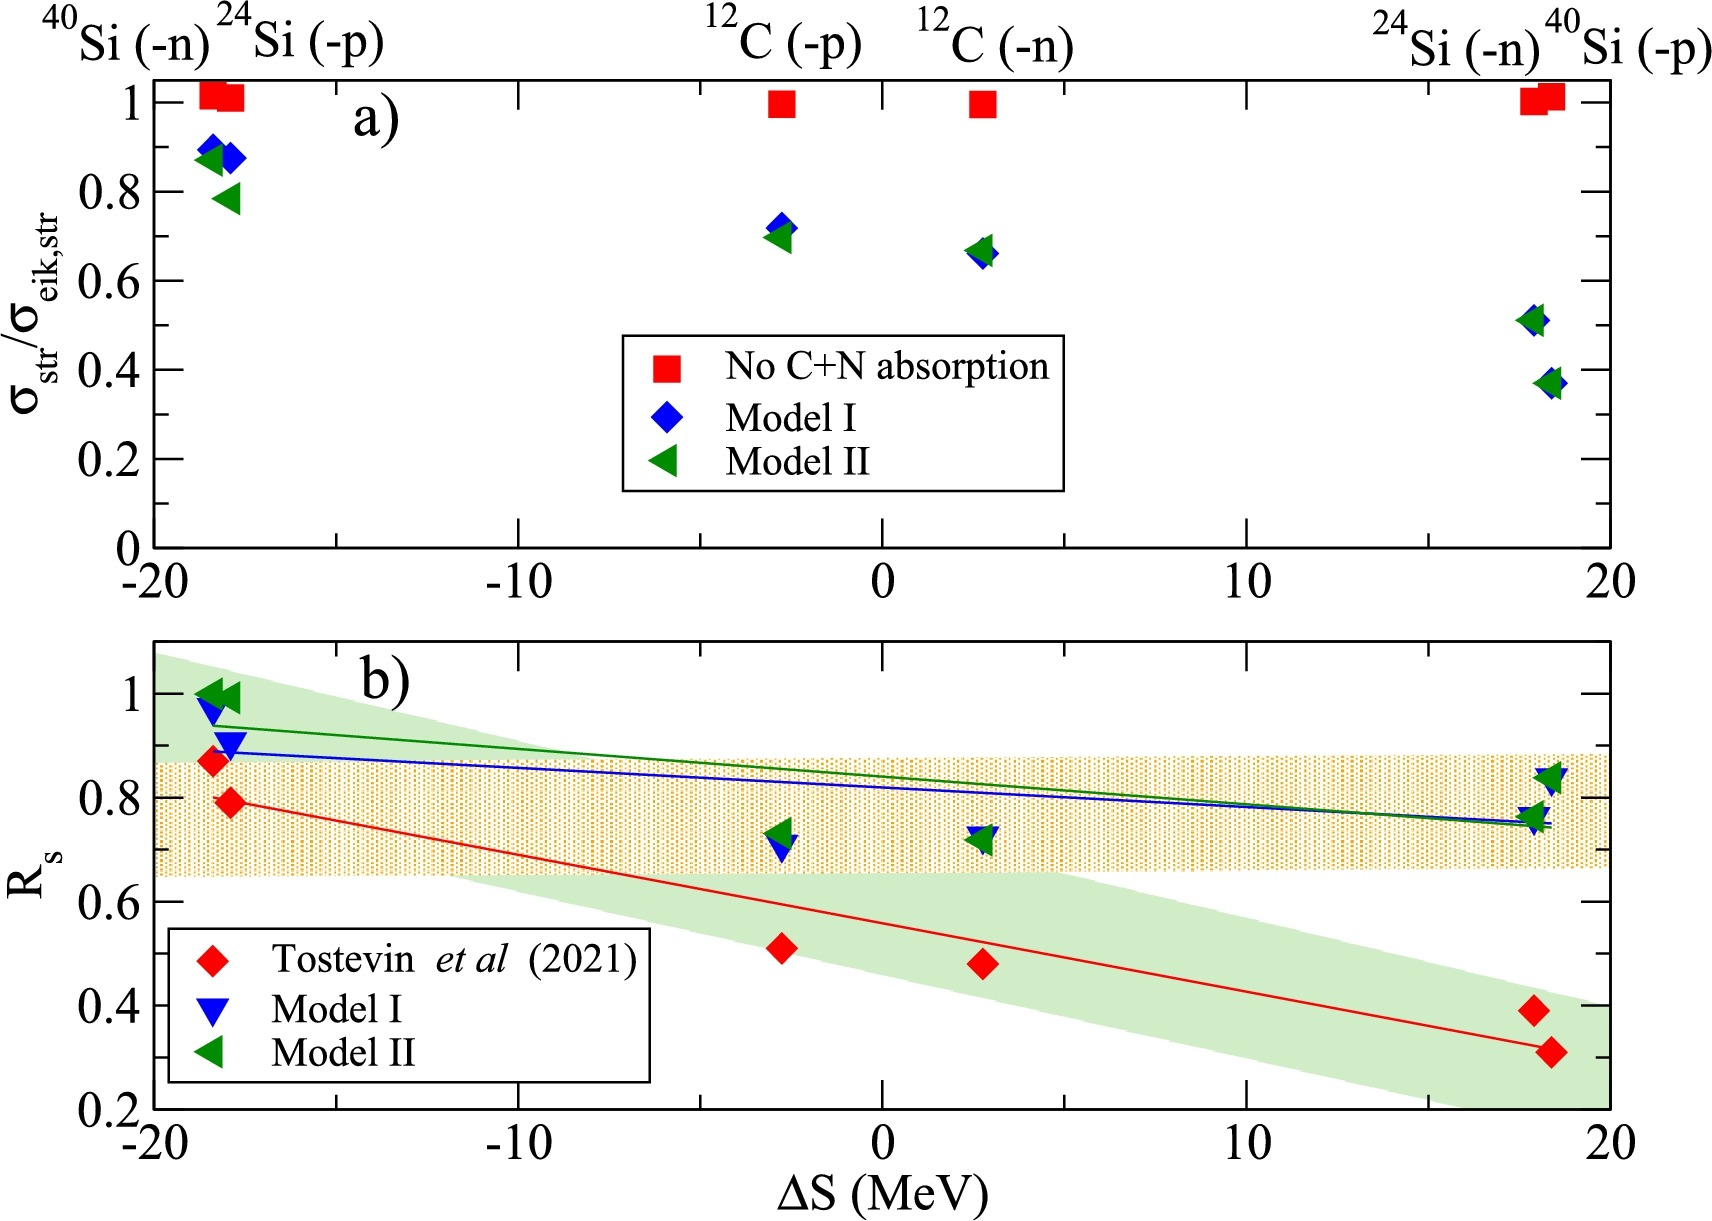
\includegraphics[height=0.3\textheight]{quenching.jpg}
    \end{minipage}
    \begin{minipage}{0.45\textwidth}
    \tiny
    \begin{itemize}
    \item Desarrollo de TC para $(p,pN)$
    \begin{itemize}
       \tiny
    \item Publicaciones teóricas
    
    PRC \textbf{97} 024608 (2018), PLB \textbf{785} 511 (2018), PRC \textbf{102} 064613 (2020)  
    
    \item Colaboraciones experimentales
    
    RIKEN: PRC \textbf{104} 044331 (2021), PRL \textbf{130} 172501 (2023), PRC \textbf{109} 034312 (2024)    
    
    \end{itemize}
    \item Aplicación a núcleos borromeos
    \begin{itemize}
    \tiny
    \item Publicaciones teóricas
    
    PLB \textbf{767} 307 (2017), PLB \textbf{772} 115 (2017), PLB \textbf{793} 13 (2019)    
    
    \item Colaboraciones experimentales
    
     RIKEN: PLB \textbf{797}, 134843 (2019)   
    
    \end{itemize}
    \item Problema de los ``quenching factors''
    
    \begin{itemize}
    \tiny
    \item Publicaciones teóricas
    
    PPNP \textbf{118} 103847 (2021), PLB \textbf{832} 137252 (2022), PLB \textbf{847} 138284 (2023)
\end{itemize}        
    
    \end{itemize}
    \end{minipage}
    
\end{frame}

\begin{frame}{Líneas de investigación} 

\large \ding{90}  L1: \underline{Reacciones de arranque de una partícula:} \underline{reacciones $(p, pN )$, knockout y transferencia}

\normalsize
    
\begin{itemize}
\item Estudio de los efectos de absorción valencia-core en reacciones de \textit{knockout}
\begin{itemize}
\item Extensión a más núcleos medidos
\item Teoría para otros observables (distribución de momentos)
\item Análisis de incertidumbres (potenciales ópticos)
\item Formalismo puramente cuántico
\end{itemize}

\item Colaboración en experimentos futuros [$(p,pN)$] (proposals, análisis)
\item Uso de extrapolaciones para evitar inestabilidades numéricas (IA?)
\end{itemize}    
    
\end{frame}

\begin{frame}{Líneas de investigación} 

\large \ding{90}  L2: \underline{Reacciones de arranque de dos partículas: reacciones $(p, 3p)$} 

\normalsize
\begin{center}    
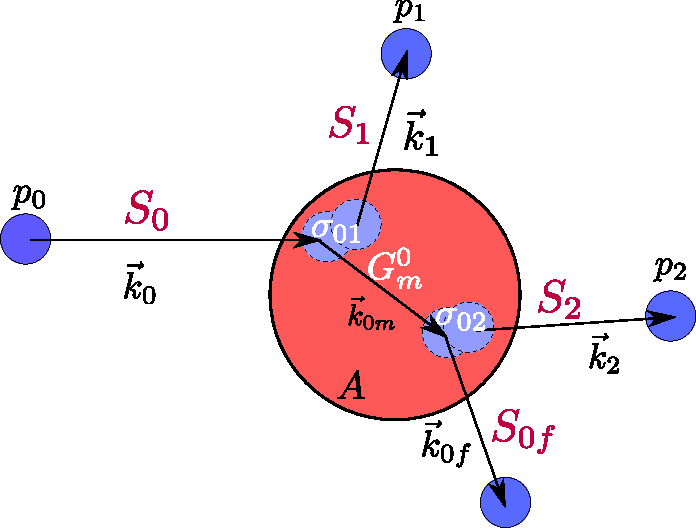
\includegraphics[height=0.5\textheight]{model.pdf}   
\end{center}
    
\end{frame}


\begin{frame}{Experiencia previa} 

   \begin{minipage}{0.45\textwidth}
    \ding{212} \tiny L2: \underline{Reacciones de arranque de dos partículas:} \underline{reacciones $(p, 3p)$} 
    
    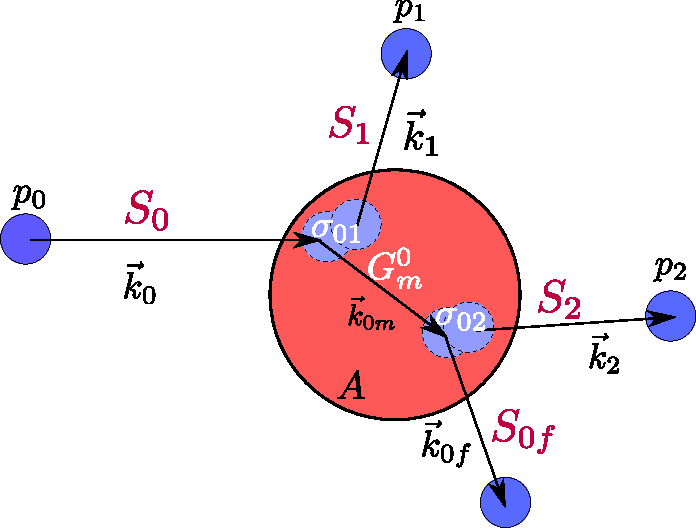
\includegraphics[height=0.3\textheight]{model.pdf}
    
    \end{minipage}
    \begin{minipage}{0.45\textwidth}
    \tiny
    \begin{itemize}
    \item Estudio de correlaciones en núcleos Borromeos
    \begin{itemize}
       \tiny
    \item Publicaciones teóricas
    
    PRC \textbf{104} 024618 (2021)
    
    \item Colaboraciones experimentales
    
    RIKEN: PLB \textbf{840} 137875 (2023)
    
    \end{itemize}
    \item Estudio de reacciones $(p,3p)$
    \begin{itemize}
    \tiny
    \item Publicaciones teóricas
    
    PRC \textbf{109} 064622 (2024)
    
    \item Colaboraciones experimentales
    
     RIKEN: PRL \textbf{125} 012501 (2020)   
    
    \end{itemize}
    \end{itemize}
    \end{minipage}
    
\end{frame}

\begin{frame}{Líneas de investigación} 

\large \ding{90} L2: \underline{Reacciones de arranque de dos partículas: reacciones $(p, 3p)$} 

\normalsize
    
\begin{itemize}
\item Colaboración en experimentos ($^X$Ar,$^X$Cl ongoing)
\item Teoría para otros observables (distribución de momentos)
\item Formalismo cuántico
\item Comparativa con reacciones de transferencia de dos protones

\end{itemize}    
    
\end{frame}

\begin{frame}{Líneas de investigación} 

\large \ding{90}  L3: \underline{Desarrollo de la teoría de reacciones a bajas energías} 

\normalsize
\begin{center}    
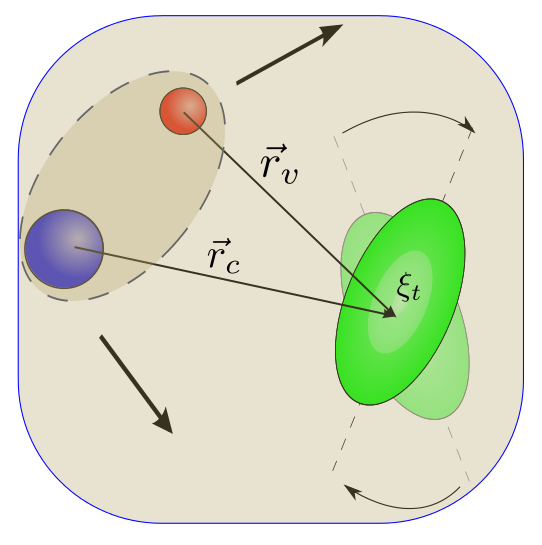
\includegraphics[height=0.3\textheight, width=\textwidth, keepaspectratio]{TExc.png}
\end{center}
    
\end{frame}

\begin{frame}{Experiencia previa} 

   \begin{minipage}{0.45\textwidth}
    \tiny\ding{212}   L3: \underline{Desarrollo de la teoría de reacciones a bajas}  \underline{ energías}   
    
    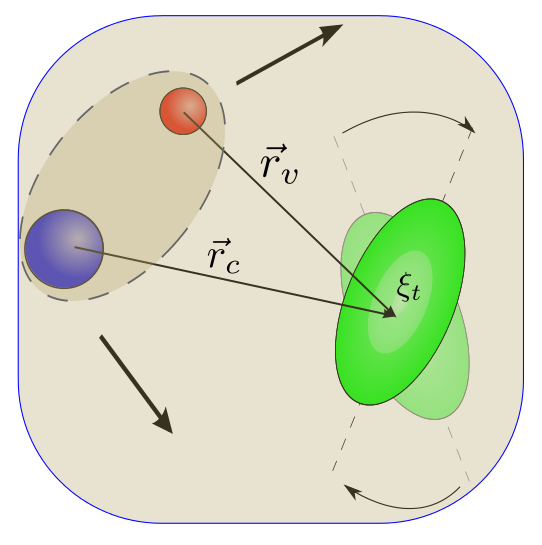
\includegraphics[height=0.3\textheight, width=\textwidth, keepaspectratio]{TExc.png}
    \end{minipage}
    \begin{minipage}{0.45\textwidth}
    \tiny
    \begin{itemize}
    \item Estudio de excitaciones colectivas
    \begin{itemize}
       \tiny
    \item Publicaciones teóricas
    
    PRC \textbf{92} 014613 (2015), PRC \textbf{95} 034609 (2017), PRC \textbf{95} 044612 (2017)
    
    \item Colaboraciones experimentales
    
    LAFN-USP: PRC \textbf{106} 014622 (2022)
    
    \end{itemize}
    \item No-localidad
    \begin{itemize}
    \tiny
    \item Publicaciones teóricas
    
    PRC \textbf{98} 011601(R) (2018),  JPG \textbf{46} 085102 (2019)
    
    \end{itemize}
    \end{itemize}
    \end{minipage}
    
\end{frame}



\begin{frame}{Líneas de investigación} 

\large \ding{90}  L3: \underline{Desarrollo de la teoría de reacciones a bajas energías} 

\normalsize
    
\begin{itemize}
\item Excitación de core y/o blanco con sistemas de tres cuerpos
\item Potenciales no locales
\begin{itemize}
\item Potenciales microscópicos \textit{ab initio}
\item Aplicación a NEB con partículas $\alpha$
\end{itemize}


\end{itemize}    
    
\end{frame}

\begin{frame}{Líneas de investigación} 

\large \ding{90}  L4: \underline{Apoyo teórico a la comunidad experimental:} \underline{desarrollo de herramientas de acceso abierto} 

\normalsize
    
\begin{itemize}
\item Participación en análisis y proposals ($^7$Be$(d,p)^8$Be$^*$;$^{70}$Zn,$^{10}$Be$(p,3p)$ activas)
\item Contribución a código abierto de reacciones del grupo de la US: THOx
\begin{itemize}
\item Absorción core-valencia
\item Dependencia del ángulo interno del deuterón
\item Cálculo exacto de estados ligados
\item Probabilidad de excitación magnética $B(M\lambda)$
\end{itemize}

\item Proyecto EUROLABS (Reaction4Exp)


\includegraphics[height=0.2\textheight]{eurolabs.jpg}   

\end{itemize}    
    
\end{frame}

\subsection{Planteamientos docentes}
\begin{frame}{Planteamientos docentes}
    \begin{block}{Perfil docente}
        \textbf{Física Nuclear y de Partículas} (Grado en Física, Doble Grado en Física e Ingeniería
de Materiales, Doble Grado en Física y Matemáticas)/Introducción a las reacciones
nucleares (Master Universitario en Física Nuclear)
    \end{block}
    \begin{itemize}
        \item Física Nuclear y de Partículas (6 ECTS) impartida en la Facultad de Física
        \item Área responsable: Física Atómica, Molecular y Nuclear
        \item Espacio Europeo de Educación Superior (EEES)
    \end{itemize}
\end{frame}

\begin{frame}{Metodología}
    \begin{itemize}
        \item Clase magistral participativa
        \item Clase de resolución de problemas
        \item Clase de resolución de dudas
        \item Tutorías
        \item Recursos digitales
    \end{itemize}
\end{frame}

\begin{frame}{Evaluación}
    \begin{itemize}
        \item Evaluación continua
        \begin{itemize}
        \item Dos controles correspondientes a los dos bloques (Física Nuclear y Física de Partículas)
        \begin{itemize}
        \item Ambos deben aprobarse para aprobar la asignatura
        \item Bloque aprobado se guarda en primera convocatoria oficial
        \end{itemize}
        \item Dos tests de respuesta múltiple de 15 min en cada bloque
        \begin{itemize}
        \item Objetivo: Incentivar el seguimiento de la asignatura
        \item Sólo puntúan tras aprobar por evaluación continua
        \end{itemize}         
        \end{itemize}
        \item Convocatoria oficial
    \end{itemize}
\end{frame}

\begin{frame}{Ejemplos preguntas tests}

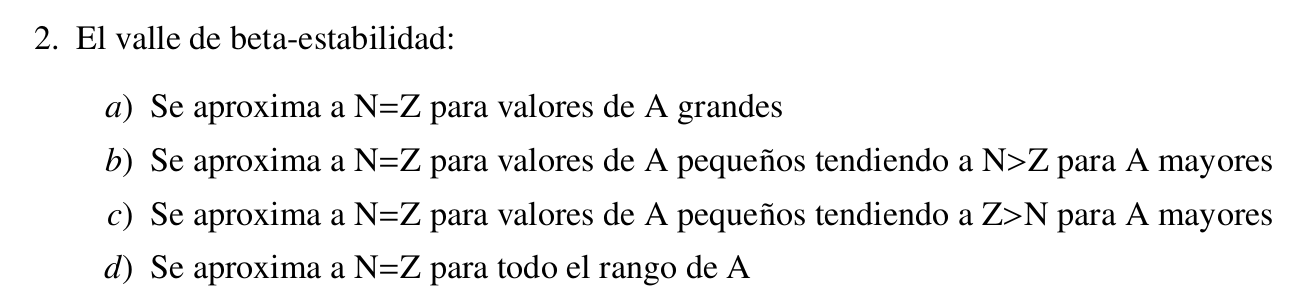
\includegraphics[width=0.7\textwidth]{test1.png}

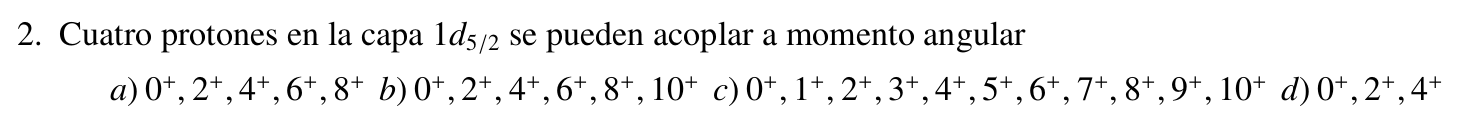
\includegraphics[width=0.8\textwidth]{test2.png}

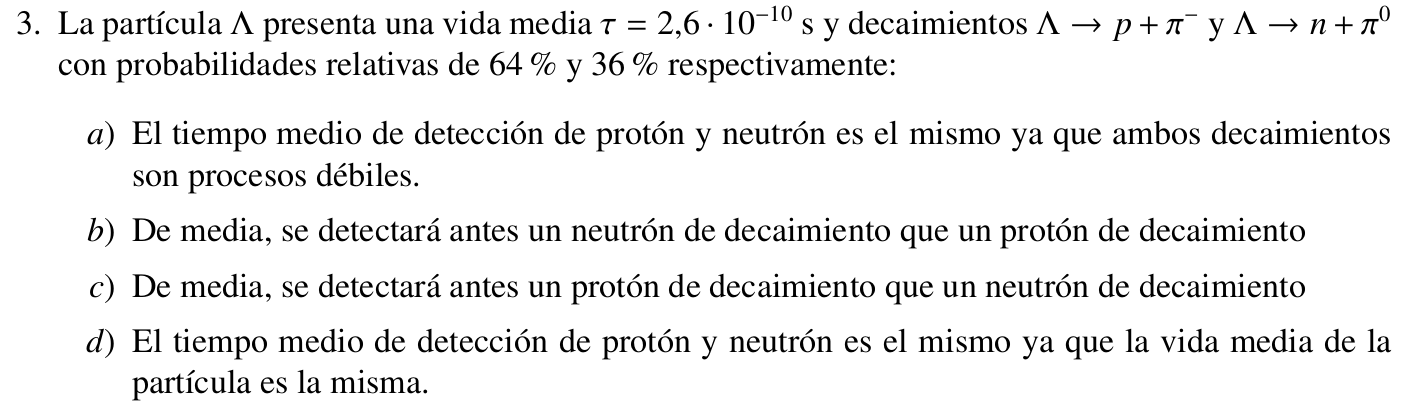
\includegraphics[width=0.7\textwidth]{test3.png}

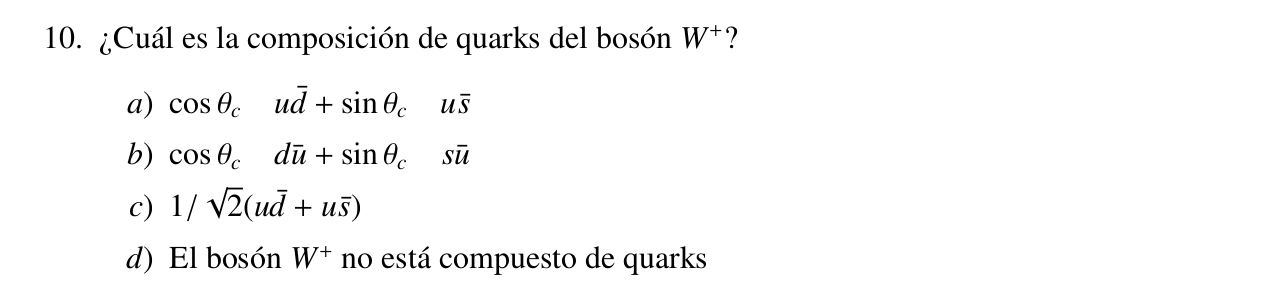
\includegraphics[width=0.8\textwidth]{test4.png}
\end{frame}

% Sección 3: Programa
\section{Programa: Física Nuclear y de Partículas}
\subsection{Temario}
\begin{frame}{Temario}
    \begin{Large}Física Nuclear\end{Large}
    \begin{itemize}
        \item Introducción a la Física Nuclear
\begin{itemize}
        \item L1.1: Introducción
\end{itemize}        
        \item Masas nucleares
\begin{itemize}
        \item L2.1: Fenomenología de las masas atómicas
        \item L2.2: Fórmula semiempírica de masas
        \item L2.3: Límites de formación nuclear
\end{itemize} 
        \item Estabilidad nuclear
\begin{itemize}
        \item L3.1: Introducción y decaimiento alfa   
        \item L3.2: Decaimiento por fisión y beta (I)
        \item L3.3: Decaimiento beta (II)
\end{itemize}      
    \end{itemize}
\end{frame}

\begin{frame}{Temario}
    \begin{itemize}
        \item Tamaños nucleares
\begin{itemize}
        \item L4.1: Medida del tamaño nuclear
        \item L4.2: Reacciones de dispersión elástica de electrones
        \item L4.3: Densidad de carga nuclear
\end{itemize}        
        \item Modelo de capas
\begin{itemize}
        \item L5.1: Introducción al modelo de capas
        \item L5.2: Modelo de partículas independientes
        \item L5.3: Aplicaciones del modelo de capas
\end{itemize} 
        \item Decaimiento gamma
\begin{itemize}
        \item L6.1: Introducción al decaimiento gamma   
        \item L6.2: Reglas de selección y unidades Weisskopf
\end{itemize} 
        \item El deuterón
\begin{itemize}
        \item L7.1: El deuterón
\end{itemize}      
    \end{itemize}
\end{frame}

\begin{frame}{Temario}
    \begin{Large}Física de Partículas\end{Large}
    \begin{itemize}
        \item Introducción a la física de partículas
\begin{itemize}
        \item L8.1: Introducción
\end{itemize}        
        \item Decaimiento y colisiones de partículas subatómicas
\begin{itemize}
        \item L9.1: Fundamentos del decaimiento de las partículas
        \item L9.2: Decaimiento débil
        \item L9.3: Secciones eficaces e interacciones fundamentales
\end{itemize} 
        \item Propiedades de las partículas subatómicas
\begin{itemize}
        \item L10.1: Teoría de Yukawa y clasificación
        \item L10.2: Extrañeza
        \item L10.3: Conservación de números cuánticos y resonancias
        \item L10.4: Isospín
\end{itemize}      
    \end{itemize}
\end{frame}

\begin{frame}{Temario}
    \begin{itemize}
        \item Simetrías discretas
\begin{itemize}
        \item L11.1: Introducción a las simetrías discretas
        \item L11.2: Simetrías P y C
\end{itemize}        
        \item Un paradigma de transición
\begin{itemize}
        \item L12.1: Introducción (somera) a la teoría cuántica de campos
        \item L12.2: Lagrangianos de interacción
        \item L12.3-4: Diagramas de Feynman 
\end{itemize} 
        \item Modelo de quarks
\begin{itemize}
        \item L13.1: Modelo de quarks dentro del grupo SU(3)
        \item L13.2: Descripción de los hadrones en la teoría de quarks
        \item L13.3: Propiedades de las partículas en el modelo de quarks y quarks pesados
        \item L13.4: Diagramas de Feynman en el modelo de quarks
\end{itemize} 
        \item Modelo estándar
\begin{itemize}
        \item L14.1: Introducción al modelo estándar
\end{itemize}      
    \end{itemize}
\end{frame}
\subsection{Bibliografía}
\begin{frame}{Bibliografía}
    \begin{itemize}
        \item Heyde, Kris L. G, \textit{Basic ideas and concepts in nuclear physics: an introductory approach}, Bristol, [England] ; Philadelphia : Institute of Physics Pub., 3rd ed., 2004, ISBN: 9780750309806
        \item Krane, Kenneth S., \textit{Introductory Nuclear Physics}, Ed. John Wiley and Sons, 2nd
ed., 1988, ISBN: 0-471-80553-X
\item David J. Griffiths, \textit{Introduction to elementary particles}, Ed. Wiley-Vch, 2008, ISBN:
978-84-344-0491-5
\item J. Gómez Camacho, \textit{Física de Partículas en 3 créditos}, Universidad de Sevilla. \url{https://idus.us.es/server/api/core/bitstreams/80552150-5cee-40d0-b973-59b3f7cd04a8/content}
    \end{itemize}
\end{frame}

% Diapositiva final
\begin{frame}{Gracias}
    \centering
    \Huge ¡Gracias por su atención!
\end{frame}

\end{document}
